\begin{figure}[H]
    \centering
    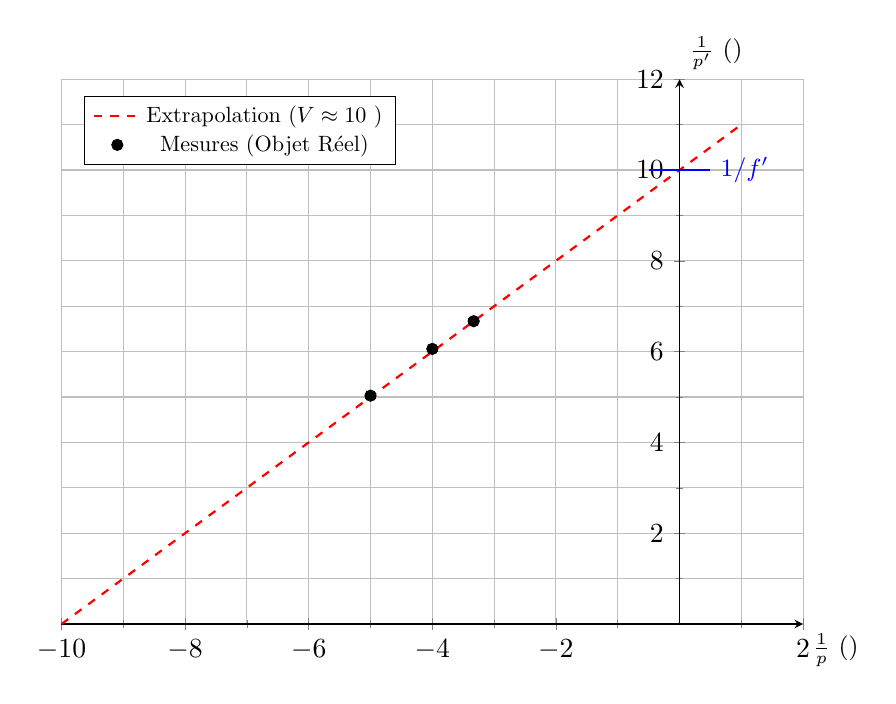
\begin{tikzpicture}
    \begin{axis}[
        axis lines = middle,
        xlabel = {$\frac{1}{p}$ (\unit{\per\meter})},
        ylabel = {$\frac{1}{p'}$ (\unit{\per\meter})},
        label style={font=\small},
        grid = both,
        minor tick num=1,
        xmin=-10, xmax=2,
        ymin=0, ymax=12,
        width=11cm, height=8.5cm,
        xlabel style={at={(ticklabel* cs:1)}, anchor=north west},
        ylabel style={at={(ticklabel* cs:1)}, anchor=south west},
        legend pos=north west,
        legend style={nodes={scale=0.8, transform shape}}
    ]

    % --- Extrapolation théorique ---
    \addplot[
        domain=-10:1,
        samples=2,
        thick,
        red,
        dashed,
    ] {x + 10};
    \addlegendentry{Extrapolation ($V \approx 10$ \unit{\per\meter})}

    % --- Points mesurés (Objet Réel) avec barres d'erreur ---
    \addplot[
        only marks,
        mark=*,
        black,
        error bars/.cd,
        y dir=both, y fixed=0.05,
        error mark options={rotate=90, mark size=2pt, line width=0.5pt}
    ]
    coordinates {
        (-5, 5.03)
        (-4, 6.06)
        (-3.33, 6.67)
    };
    \addlegendentry{Mesures (Objet Réel)}

    % --- Marquage de l'ordonnée à l'origine ---
    \draw[blue, thick] (axis cs:-0.5,10) -- (axis cs:0.5,10) node[right] {\small $1/f'$};

    \end{axis}
    \end{tikzpicture}
    \caption{Détermination de la vergence par exploitation de la relation de conjugaison.}
    \label{fig:graphe_focometrie}
\end{figure}